\documentclass{standalone}
\usepackage{tikz}


\begin{document}

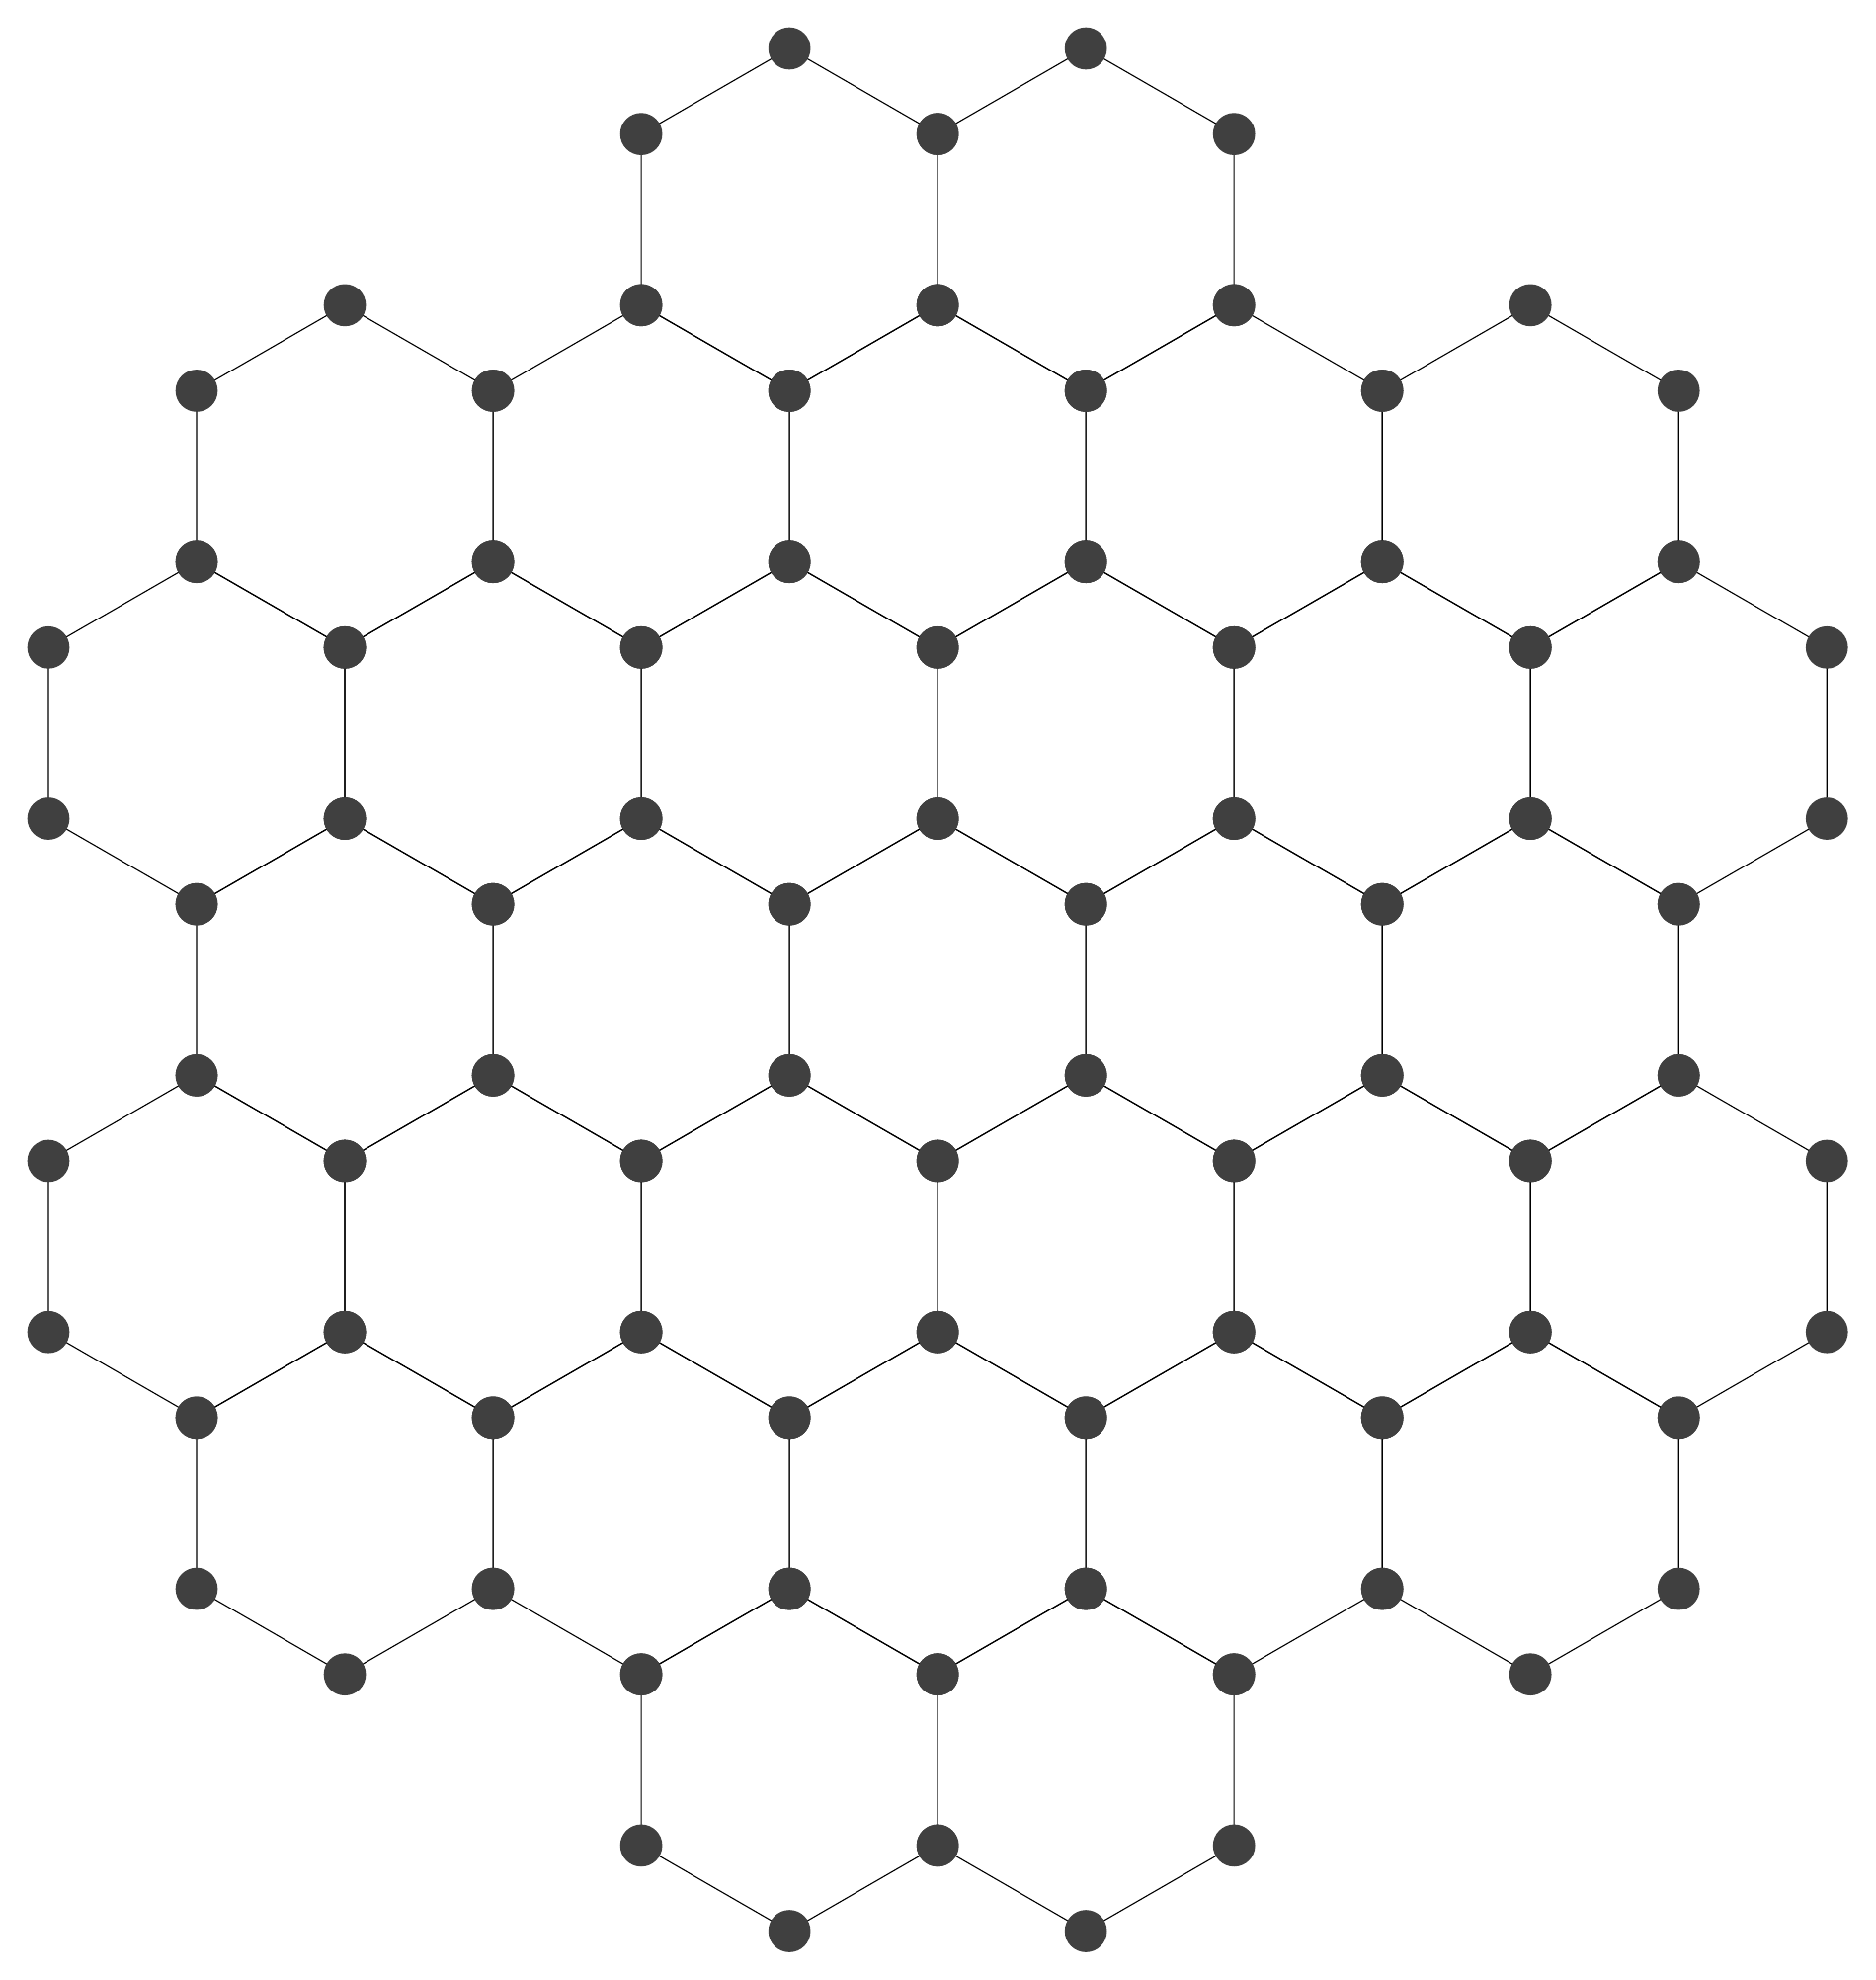
\begin{tikzpicture}[scale=2.2]
\def\hex#1#2{
  \draw #1 #2 +(30:1) \foreach \a in {90,150,...,330} { -- +(\a:1) } -- cycle;
  \draw[darkgray,fill=darkgray] #1 #2 \foreach \a in {30,90,...,330} { +(\a:1) circle (1.2mm) } ;
}
\def\distanceamongcells{1.732050}
\def\hexblue#1#2{
  \draw[blue!40,very thick] #1 #2 +(0:\distanceamongcells) \foreach \a in {60,120,...,300}
     { -- +(\a:\distanceamongcells) } -- cycle;
}
    % Draw grid of small hexagons
\hex{(0,0)}{(0,0)}
\foreach \a in {0,60,...,300} {\hex{ (0,0)}{(\a:\distanceamongcells)}}
\foreach \a in {0,60,...,300} {\hex{ (0,0)}{(\a:2*\distanceamongcells)}}
\foreach \a in {30,90,...,330} {
  \hex{(0,0)}{(\a:3)}
  \hex{(\a:3)}{++(\a-30:\distanceamongcells)}
  \hex{(\a:3)}{++(\a+30:\distanceamongcells)}
  % \fill[red!40!black] (\a:3) circle(2mm);
}
\end{tikzpicture} 



\end{document}
